\section{Inequalities for Entropy and Mutual Information}
\subsection{Convexity and Jensen's Inequality}

\begin{remark}
    We use the common definition of convex functions and concave functions from analysis.
\end{remark}

\begin{theorem}[Jensen's Inequality]
    Let $\mathcal{X} \subset \mathbb{R}$, $f: \mathcal{X} \rightarrow \mathbb{R}$ a function. Let $\mathbb{E} f(X)$ and $f(\mathbb{E} X)$ be defined.
    \begin{enumerate}
        \item If $f$ is convex, we have $\mathbb{E} f(X) \ge f(\mathbb{E} X)$.
        \item If $f$ is concave, we have $\mathbb{E} f(X) \le f(\mathbb{E} X)$.
        \item If $f$ is strictly convex and $\mathbb{E} f(X) = f(\mathbb{E} X)$, then $X = \mathbb{E}[X]$ almost surely.
    \end{enumerate}
\end{theorem}
\begin{proof}
    \begin{enumerate}
        \item
            Let $n \in \mathbb{N} \setminus \{1\}$ and, without loss of generality, assume that $p_1, \cdots, p_n \in (0, 1)$ satisfy $\sum_{i=1}^{n}{p_i} = 1$ and $x_1, \cdots, x_n \in \mathbb{R}$.
            Distinguish two cases. If $\mathcal{X}$ is finite:
            We show $f\paren{\sum_{i=1}^{n}{p_i x_i}} \le \sum_{i=1}^{n}{p_i f(x_i)}$ by induction. \\
            The definition of convexity yields the base case $i = 2$: $f(p_1 x_1 + p_2 x_2) \le p_1 f(x_1) + p_2 f(x_2)$. \\
            We assume the claim holds for $n - 1$ and the induction case goes as follows: \\
            \begin{align*}
                f\paren{\sum_{i=1}^{n}{p_i x_i}} &= f\paren{p_1 x_1 + (1 - p_1) \sum_{i=2}^{n}{\frac{p_i}{1 - p_1} x_i}} \\          
                &\le p_1 f\paren{x_1} + (1 - p_1) f\paren{\sum_{i=2}^{n}{\frac{p_i}{1 - p_1} x_i}}              && \text{(def. of convexity)} \\
                &\le p_1 f\paren{x_1} + (1 - p_1) \sum_{i=2}^{n}{\frac{p_i}{1 - p_1} f\paren{{x_i}}}         
                && \text{(induct. hypo. applies since $\sum_{i = 2}^{n}{\frac{p_i}{1 - p_1}}$ = 1)} \\
                &= \sum_{i=1}^{n}{p_i f\paren{{x_i}}}
            \end{align*}
            Else: If $\mathcal{X}$ is countably infinite, the claim follows using the limit of the previous case.

        \item
            Follows from part 1 applied to $-f$.

        \item
            If the support of $X$ has more than one element, the inequality in part 1 is strict since $f$ is strictly convex.
            This contradicts the assumption $\mathbb{E} f(X) = f(\mathbb{E} X)$.
            Hence $X = c$ almost surely for some constant $c$.
            By definition of the expectation, this constant must be $c = \mathbb{E}[X]$.
    \end{enumerate}
\end{proof}

\begin{corollary}
    Entropy and Mutual Information are non-negative:
    \begin{enumerate}
        \item $0 \le H(X)$
        \item $0 \le D(p \| q)$
        \item $0 \le I(X; Y)$
    \end{enumerate}
\end{corollary}
\begin{proof}
    \begin{enumerate}
        \item 
            Note that $\log(\frac{1}{[0, 1]}) = \log([1, \infty]) = [0, \infty]$ 
            and $p_X(X) \in [0, 1]$. \\
            Using the monotonicity of the expected value, we obtain
            \[
                0 \le \mathbb{E}\paren{\log \paren{\frac{1}{p_X(X)}}}
                = -\mathbb{E}\paren{\log \paren{p_X(X)}} = H(X)
            \]

        \item 
            We can prove this using Jensens Inequality on a \textit{concave} function: % TODO: Make sure we use the support correctly.
            Let $X \sim p$. 
            \begin{align*}
                -D(p \| q) &= -\mathbb{E}_{p}\paren{\log \frac{p(X)}{q(X)}}
                = \mathbb{E}_{p}\paren{\log \frac{q(X)}{p(X)}}                          && \text{(def. of relative entropy)}            \\
                &\le \log\paren{\mathbb{E}_{p} \frac{q(X)}{p(X)}}                      && \text{(apply Jensen's inequality)} \\
                &= \log\paren{\sum_{x \in \supp(p)}{p(x) \frac{q(x)}{p(x)}}}
                = \log\paren{\sum_{x \in \supp(p)}{q(x)}}                              && \text{(def. of exp. value, simplify expr.)}  \\
                &\le \log\paren{\sum_{x \in \mathcal{X}}{q(x)}} = \log\paren{1} = 0 && \text{(q is a prob. function)}
            \end{align*}
            So $-D(p \| q) \le 0$, hence $D(p \| q) \ge 0$.
        \item Follows from part 2: $I(X; Y) = D(p_{X,Y} \| p_X p_Y) \ge 0$.
    \end{enumerate}
\end{proof}


\subsection{Additional Properties of Entropy}
\begin{figure}[t]
    \centering
    \begin{subfigure}[b]{0.45\textwidth}
        \centering
        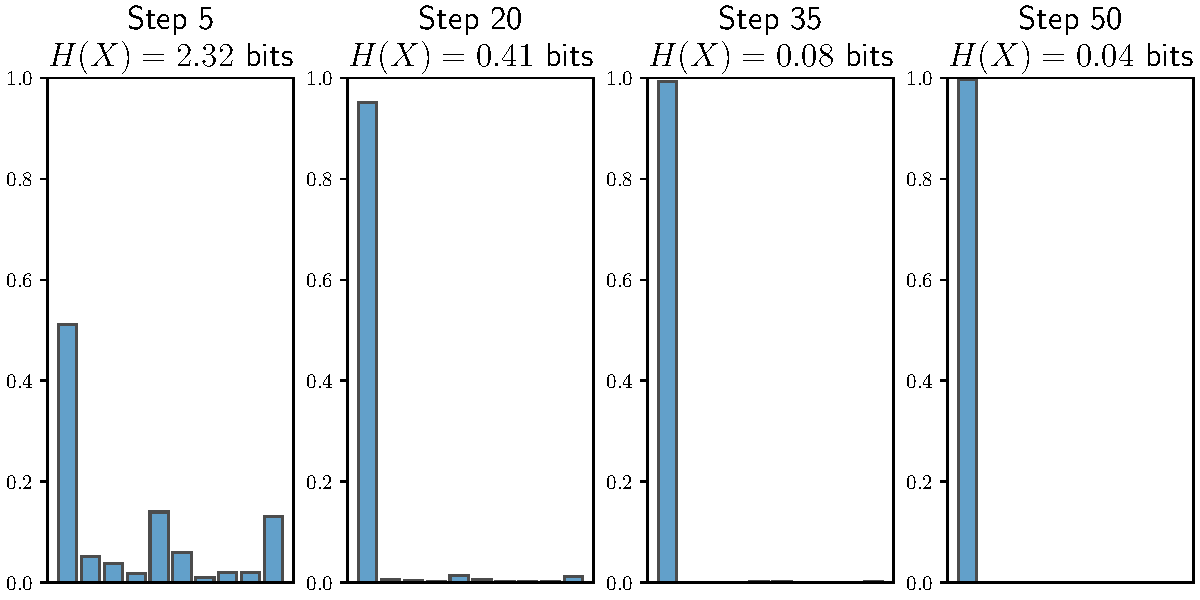
\includegraphics[width=1.0\linewidth]{../plots/peak_distribution_minimises_entropy.pdf}
        \caption{Peak Distribution minimises Entropy}
        \label{fig:peak-distr-min-entropy}
    \end{subfigure}
    \hfill
    \begin{subfigure}[b]{0.45\textwidth}
        \centering
        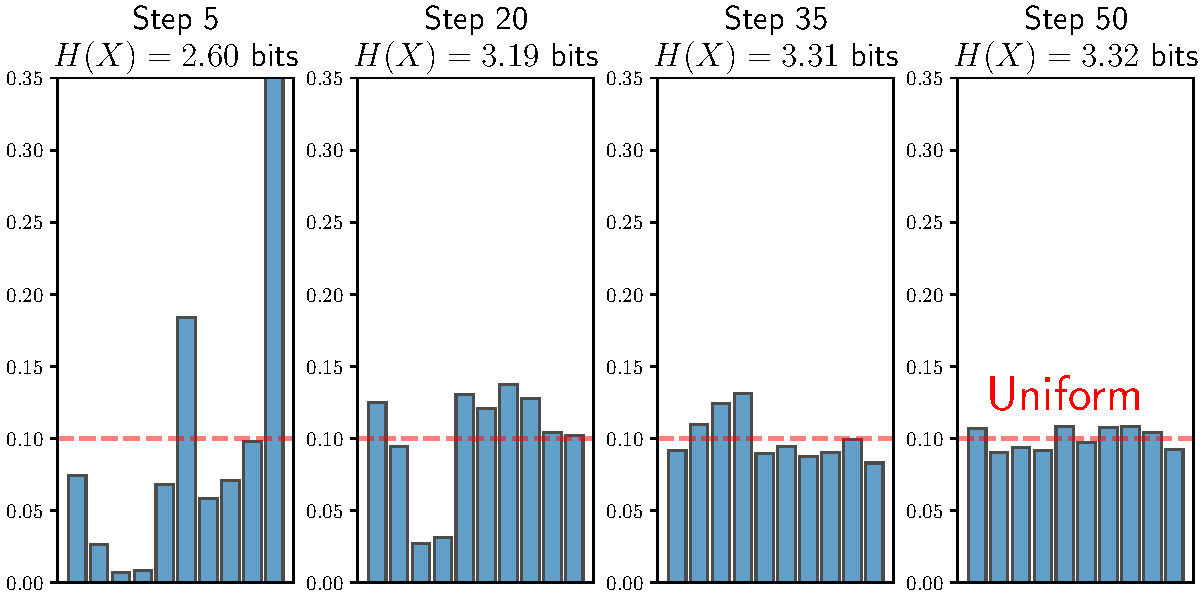
\includegraphics[width=1.0\linewidth]{../plots/uniform_distribution_maximises_entropy.pdf}
        \caption{Uniform Distribution maximises Entropy}
        \label{fig:uniform-distr-max-entropy}
    \end{subfigure}
\end{figure}

\begin{remark}
    There are multiple natural questions we can ask about Entropy.
    We will look at an example for each of them and then prove the results in the follow-up theorem.
    \begin{enumerate}
        \item Can conditioning on more information increase the entropy? \\
            Figure \ref{fig:relationships-entropy-mutual-information} illustrates the idea, that conditioning on more information can never increase the entropy.
            We will prove this exact statement: $H(X \mid Y) \le H(X)$.

        \item What distribution maximises the value of Entropy? \\
            To get a computational intuition for this question, we need to limit our random variables to finite supports.
            Let $X_p \sim \mathrm{Categorical}(p_1, \cdots, p_n)$ be a categorical distribution. \\
            We can now write the question as an optimisation problem:
            \[
                \max_{p \in \mathbb{R}^{n}, \|p\|_1=1, p \ge 0}{H(X_p)}
            \]
            The constraints can be automatically achieved by passing the logits through a \textit{Softmax} function.
            We start from a random initialisation.
            Figure \ref{fig:uniform-distr-max-entropy} illustrates the process of solving the problem using Gradient Descent using Tinygrad \cite{Tinygrad}.
            From the data, it seems plausible that the uniform distribution maximises entropy.
            We will prove this statement.

        \item What distribution minimises the value of Entropy? \\
            Figure \ref{fig:peak-distr-min-entropy} suggests that a peaked distribution minimises entropy.
            The setup is analogous to the previous optimisation problem and the figure was generated in the same way using Tinygrad.
            We will prove the statement
            \[
                H(X) = 0 \iff \exists x \in \mathcal{X}: p_X(x) = 1.
            \]

        \item What happens to the Entropy if we add independent noise to our measurements? \\
            Let $X \sim U(\{1, 2, 3, 4\})$ be the original signal, $N \sim U(\{0, 1\})$ the noise and let $X, N$ be independent. 
            Then $S \defeq X + N$ is a noisy signal. We expect the entropy to never decrease. We will prove this later.

    \end{enumerate}
\end{remark}

\begin{theorem} \label{theorem:more-entropy-observations}
    We can formalise the previous observations including some more:
    \begin{enumerate}
        \item More information can only \textit{decrease} entropy:
            \[
                H(X \mid Y) \le H(X)
            \]
        \item A peaked distribution minimises entropy:
            \[
                H(X) = 0 \iff \exists x \in \mathcal{X}: p_X(x) = 1
            \]
        \item The uniform distribution maximizes entropy:
            \[
                H(X) \le \log |\mathcal{X}| \text{ and } H(X) = \log |\mathcal{X}| \iff X \sim U(\mathcal{X})
            \]
        \item If $Y$ is determined by $X$, then:
            \[
                H(Y \mid X) = 0 \implies \exists f\vcentcolon Y = f(X) \; \text{almost surely}
            \]
        \item If independent noise is added to a random variable, entropy can only increase:
            Set $Z = X + Y$. Then we have
            \[
                X, Y \text{independent} \implies H(X) \le H(Z) \land H(Y) \le H(Z)
            \]
        \item The joint entropy of many variables never exceeds the sum of the individual entropies:
            \[
                H(X_1, \cdots, X_n) \le \sum_{i=1}^{n}{H(X_i)}
            \]
    \end{enumerate}
\end{theorem}
\begin{proof}
    \begin{enumerate}
        \item
            \[
                0 \le I(X; Y) = H(X) - H(X \mid Y) \iff H(X \mid Y) \le H(X)
            \]

        \item
            We have
            \[
                H(X) = \sum_{x \in \mathcal{X}} -p_X(x) \log p_X(x).
            \]
            Each summand is non-negative, so $H(X) = 0$ holds if and only if
            \[
                \forall x \in \mathcal{X}: -p_X(x) \log p_X(x) = 0.
            \]
            For every $x \in \mathcal{X}$ with $p_X(x) > 0$, this implies $\log p_X(x) = 0$, hence $p_X(x) = 1$.
            Therefore, $H(X) = 0$ if and only if there exists $x \in \mathcal{X}$ with $p_X(x) = 1$.

        \item
            Let $Y \sim U(\mathcal{X})$ be such that $\forall x \in \mathcal{X}\vcentcolon q(x)=\frac{1}{|\mathcal{X}|}$.
            \begin{align*}
                0 &\le D(p_X \| q)
                = \mathbb{E}_{p_X}\paren{\log \frac{p_X(X)}{q(X)}}
                = \sum_{x \in \mathcal{X}}{p_X(x) \log \frac{p_X(x)}{q(x)}} \\
                &= \sum_{x \in \mathcal{X}}{p_X(x) \log\paren{p_X(x)|\mathcal{X}|}}
                = \sum_{x \in \mathcal{X}}{p_X(x) \log p_X(x)} + \log |\mathcal{X}| \sum_{x \in \mathcal{X}}{p_X(x)}\\
                &= -H(X) + \log |\mathcal{X}| = \log |\mathcal{X}| - H(X)
            \end{align*}
            This is equivalent to $H(X) \le \log |\mathcal{X}|$.
            Lastly, Jensen's Inequality gives us: $H(X) = \log |\mathcal{X}| \iff X \sim U(\mathcal{X})$.
        \item
            We have $H(Y \mid X) = -\mathbb{E}_{p_{X,Y}}\paren{\log p_{Y \mid X}(Y \mid X)} = \sum_{(x, y) \injoint}{-p_{X,Y}(x, y) \log p_{Y \mid X}(y \mid x)}$. \\
            Additionally, we have $\forall (x, y) \in \mathcal{X} \times \mathcal{Y}: -p_{X,Y}(x, y) \log p_{Y \mid X}(y \mid x) \ge 0$. \\
            Combining those facts, we get
            \begin{align*}
                H(Y \mid X) = 0
                &\iff \forall (x, y) \injoint: p_{X,Y}(x, y) \log p_{Y \mid X}(y \mid x) = 0 \\
                &\iff \forall (x, y) \injoint: p_{X,Y}(x, y) = 0 \oplus p_{Y \mid X}(y \mid x) = 1
            \end{align*}
            This tells us, that either $p_{X,Y}(x, y) = 0$ or $p_{X,Y}(x, y) = p_{Y \mid X}(y \mid x)p_X(x) = p_X(x) = 1$. \\
            Define $(y_x)_{x \in \mathcal{X}}$ such that $\forall x \in \mathcal{X}: p_{X,Y}(x, y_x) > 0$. \\
            Set $f: \supp(X) \rightarrow \mathcal{Y}, x \mapsto y_x$. This gets us $Im(f) = \{y_x: x \in \mathcal{X}\} = \{y \in \mathcal{Y}: p_{X,Y}(x, y) > 0\}$. \\
            So $Y = f(X) \; \text{almost surely}$.

        \item
            We have
            \begin{align*}
                 H(Z \mid X) &= -\mathbb{E}_{p_{X,Y}}\paren{\log p_{Z \mid X}(Z \mid X)} = \sum_{(x, y) \injoint}{-p_{X,Y}(x, y) \log \prob[Z = x + y \mid X = x]} \\
                 &= \sum_{(x, y) \injoint}{-p_{X,Y}(x, y) \log \prob[X + Y = x + y \mid X = x]} \\
                 &= \sum_{(x, y) \injoint}{-p_{X,Y}(x, y) \log \prob[Y = y \mid X = x]}
                 = -\mathbb{E}_{p_{X,Y}}\paren{\log p_{Y \mid X}(Y \mid X)} = H(Y \mid X)
            \end{align*}
            Using Independence and Information never hurts, we get
            $H(Y) = H(Y \mid X) = H(Z \mid X) \le H(Z)$.
            By an analogous argument, we get
            $H(X) = H(X \mid Y) = H(Z \mid Y) \le H(Z)$.

        \item
            Using the Chain rule, we have
            \begin{align*}
                H(X_1, \cdots, X_n) &= \sum_{i=1}^{n}{H(X_i \mid X_1, \cdots, X_{i-1})}         && \text{(chain rule)} \\
                &\le \sum_{i=1}^{n}{H(X_i)}                                                     && \text{(information never hurts)}
            \end{align*}

    \end{enumerate}
\end{proof}


\subsection{The Log-Sum Inequality}

\begin{theorem}[Log-Sum Inequality]
    Let $n \in \mathbb{N}$, $a_1, \cdots, a_n, b_1, \cdots, b_n \ge 0$.
    Then we have 
    \[
        \sum_{i=1}^{n}{a_i \log\frac{a_i}{b_i}} 
        \ge \paren{\sum_{i=1}^{n}{a_i}}\log\frac{\sum_{i=1}^{n}{a_i}}{\sum_{i=1}^{n}{b_i}}
    \]
\end{theorem}
\begin{proof}
    The proof of this inequality goes beyond the scope of the paper. Please refer to Elements of Information Theory \cite{Thomas:ElementsOfInformationTheory} for more information.
\end{proof}

\begin{theorem}[Convexity of Entropy] \label{theorem:convexity-of-entropy}
    \begin{enumerate}
        \item
            $D(. \| .)$ is a convex function. This means that
            \[
                \begin{aligned}
                \forall p_1, q_1, p_2, q_2, \forall \lambda \in [0, 1]\vcentcolon \quad
                &D(\lambda p_1 + (1-\lambda) p_2 \| \lambda q_1 + (1-\lambda) q_2) \\
                &\le \lambda D(p_1 \| q_1) + (1 - \lambda) D(p_2 \| q_2)
                \end{aligned}
            \]

        \item
            Let $X_p \sim B(1, p)$ for all $p \in (0, 1)$ and $h(p) \defeq H(X_p)$. \\
            Then $h \le 1$ and $h$ is a concave function.

    \end{enumerate}
\end{theorem}
\begin{proof}
    \begin{enumerate}
        \item
            Let $p_1, q_1, p_2, q_2$ be probability mass functions on $\mathcal{X}$.
            Let $\lambda \in (0, 1)$. \\
            First of all, the set of probability densities is convex. 
            So the above statement is well-defined. \\
            Secondly, the inequality needs to be verified:
            \begin{align*}
                &D(\lambda p_1 + (1-\lambda) p_2 \| \lambda q_1 + (1-\lambda) q_2) \\
                &= \sum_{x \in \mathcal{X}}{\paren{\lambda p_1(x) + (1-\lambda) p_2(x)} \log \frac{\lambda p_1(x) + (1-\lambda) p_2(x)}{\lambda q_1(x) + (1-\lambda) q_2(x)}}      
                && \text{(by definition)} \\
                &\le \sum_{x \in \mathcal{X}}{\lambda p_1(x) \log \frac{p_1(x)}{q_1(x)} + (1-\lambda) p_2(x) \log \frac{p_2(x)}{q_2(x)}}        && \text{(log-sum inequality on the 2 two-sums)} \\
                &= \lambda D(p_1 \| q_1) + (1-\lambda) D(p_2 \| q_2)                                                                            && \text{(by definition)}
            \end{align*}

        \item
            First, we have
            \begin{align*}
                h(p) &= H(X_p) = -p \log p - (1-p) \log (1-p)       && \text{(by definition)} \\
                &= -(p \log p + (1-p) \log (1-p))                   && \text{(factor out)} \\
                &\le -(p + 1 - p) \log \frac{p + 1 - p}{1 + 1} = -\log \frac{1}{2} = 1  && \text{(simplify)}
            \end{align*}
            Second, for $q$ with $\forall x \in \mathcal{X}: q(x)=\frac{1}{|\mathcal{X}|}$ we have
            Let $p_1, p_2 \in [0, 1]$ and $\lambda \in (0, 1)$.
            \begin{align*}
                h(\lambda p_1 + (1-\lambda) p_2) &= H(X_{\lambda p_1 + (1-\lambda) p_2})                            && \text{(by definition)} \\
                &= |\mathcal{X}| - D(\lambda p_1 + (1-\lambda) p_2 \| q)                                            && \text{(using theorem \ref{theorem:more-entropy-observations})} \\
                &\ge |\mathcal{X}| - \lambda D(p_1 \| q) - (1-\lambda) D(p_2 \| q)                                  && \text{(using convexity)} \\
                &= \lambda \paren{|\mathcal{X}| - D(p_1 \| q)} - (1-\lambda) \paren{|\mathcal{X}| - D(p_2 \| q)}    && \text{(factor out twice)} \\
                &= \lambda H(X_{p_1}) - (1-\lambda) H(X_{p_2}) = \lambda h(p_1) + (1-\lambda) h(p_2)                && \text{(by definition, simplify)} \\
            \end{align*}
    \end{enumerate}
\end{proof}
